\begin{center}
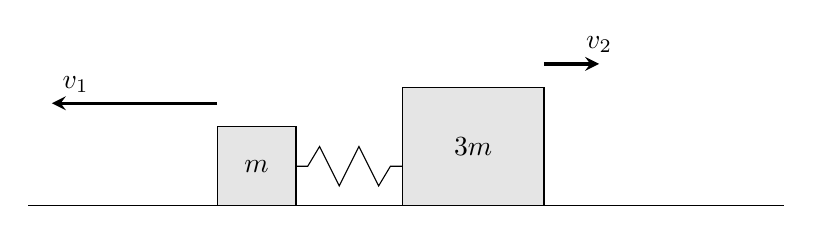
\begin{tikzpicture}[>=stealth]
 \draw (0,0) -- (9.6,0);
 \draw[fill=gray!20] (2.4,0) rectangle (3.4,1);
 \node at (2.9,0.5) {$m$};
 \draw (3.4,0.5) -- (3.55,0.5) -- (3.7,0.75) -- (3.95,0.25) -- (4.2,0.75) -- (4.45,0.25) -- (4.6,0.5) -- (4.75,0.5);
 \draw[fill=gray!20] (4.75,0) rectangle (6.55,1.5);
 \node at (5.65,0.75) {$3m$};
 \draw[->, very thick] (2.4,1.3) -- (0.3,1.3) node[above right] {$v_1$};
 \draw[->, very thick] (6.55,1.8) -- (7.25,1.8) node[above] {$v_2$};
\end{tikzpicture}
\end{center}

Vorher ruhen beide Körper, der Gesamtimpuls ist null. Danach bewegen sie sich in entgegengesetzte Richtungen, mit den Beträgen $v_1$ (Masse $m$) und $v_2$ (Masse $3m$):
\begin{align}
 0 &= m\,v_1 - 3m\,v_2 \quad\Rightarrow\quad v_1 = 3\,v_2
\end{align}
Der leichtere Körper ist also schneller, und die Geschwindigkeiten unterscheiden sich um $\Delta v = v_1 - v_2 = 2\,v_2$. Damit ist
\begin{align}
 v_2 &= \vZwF = \frac{\vDi}{2} = \vZw \approx \result{\vZwP{0}{2}} \\
 v_1 &= \vErF = \frac{3\cdot\vDi}{2} = \vEr \approx \result{\vErP{0}{2}}
\end{align}
